%!TEX root = main.tex

\section{Research Questions, Objectives, and Expected Outcomes}

Recommender systems predicts user-item interests by learning historical interaction records. Though, it is well recognized by the industry, at different stages, it still faces a number of challenges. 
To be more specific, recommender system often faces data sparsity problem in its early launching stage due to the lack of historical interactions. 
Subsequently, many recommender system also experience the limitation on new emerging data at post training stage.

In this research, we explore the combined effect of knowledge graphs representation learning and transfer learning for reducing the launching barriers of recommendation model productionisation. Further, we leverage the rich semantic information of knowledge graph to build an adaptive cross-domain recommendation framework for tackling data sparsity and cold start challenges. 

\subsection{Questions}

\subsubsection*{Question 1}
How to represent users and items in a unified heterogeneous knowledge graph for data quality improvement?

\subsubsection*{Question 2}
How to improve recommender systems' adaptiveness on new and unseen data with knowledge graph embedding?

\subsubsection*{Question 3}
How to use knowledge graphs to transfer cross-domain knowledge for enhanced recommendation results?

\subsection{Objectives}
This research aims to achieve following objectives: 

\bigskip
\textbf{Objective 1:} To develop a graph based representation method to enhance users and items embeddings in a unified heterogeneous knowledge graph for data density improvement.(Aim to answer question 1)

Collaborative Filtering (CF) based recommender systems, commonly, only uses user-item interactions records in training. Such approach ignores important user/item feature, and is unable to learn non-interacted user/item entities. 

In this objective, by leveraging the heterogeneous graph, user-item interactions, as well as users/items attributes, can be naturally projected into a single multiple-hub network \citep{Shi2017} structure. Nodes representation then can be learned holistically by traversing the meta-path of the graph. Such approach allows recommendation model to incorporate richer information from knowledge graph to reduce data sparsity and overcome the interaction limitation during training process.


\bigskip
\textbf{Objective 2:} To develop an adaptive strategy for improving recommender systems’ adaptiveness on new and unseen data with knowledge graph embedding. (Aim to answer question 2)

Commonly, recommender systems use user/item latent feature for prediction, which were trained on static datasets. For new item or user that appeared post training, their latent feature would not be known until being included in the later re-training. It is known as cold start problem.

In this study, we aim to develop a recommender system that is capable of making predictions on these unseen data points without mandatory model re-training. New entity representation is calculated inductively via knowledge graph instead of being looked up from cache for recommendation predictions.


\bigskip
\textbf{Objective 3:} To develop a cross-domain recommendation method that improves target sparse domain prediction results by transferring relative richer source domains knowledge across. (Aim to answer question 3)

Subsequent to object 1 and 2, the single domain recommender system frequently suffers from data sparsity problems in its early launching phrase. In order to alleviate the issue and assure prediction quality, our research tries to develop a knowledge transfer method, which improves data density by transferring learning from a similar but denser domain through the knowledge graph. So that, the recommender system can make high quality predictions early on.

\bigskip
\textbf{Objective 4:} To develop an adaptive cross-domain recommender system prototype with case studies for validating the suggested approaches. (Aim to answer question 1,2,3)

By putting research results from Objective 1,2,3 into a holistic framework. It would enable us to develop a generic approach and making recommendation model adapting to data changes. Such system would significantly ease the "bring to market" effort, improve prediction quality and reduce the maintenance cost over time. 

Following common datasets will be used for representation method verification: 

\begin{itemize}

\item MovieLens dataset (http://grouplens.org/datasets/movielens/) 

\item Netflix dataset (http://www.lifecrunch.biz/archives/207) 

\item DBLP Citation Networks (https://dblp.uni-trier.de)  

\end{itemize}

Further we will user real estate and job related dataset for cross-domain recommendation applications


\subsection{Expected Outcomes}

Based on research questions and objectives above, the following outcomes are expected:
1) A knowledge graph based representation learning method for dealing with cold start and data sparsity problem;
2) An knowledge graph embeddings based recommendation model that is capable of making prediction on unseen user/item input adaptively;
3) A cross-domain technique to enhance target domain recommendation model by leveraging denser source domain knowledge with transfer learning;
4) A unified adaptive cross-domain recommender system with heterogeneous knowledge graph;
5) Several high quality papers and a PhD thesis. A research overview can be depict as Fig. \ref{fig:r_overview} below: 
\begin{figure*}[!h]
    \centering
    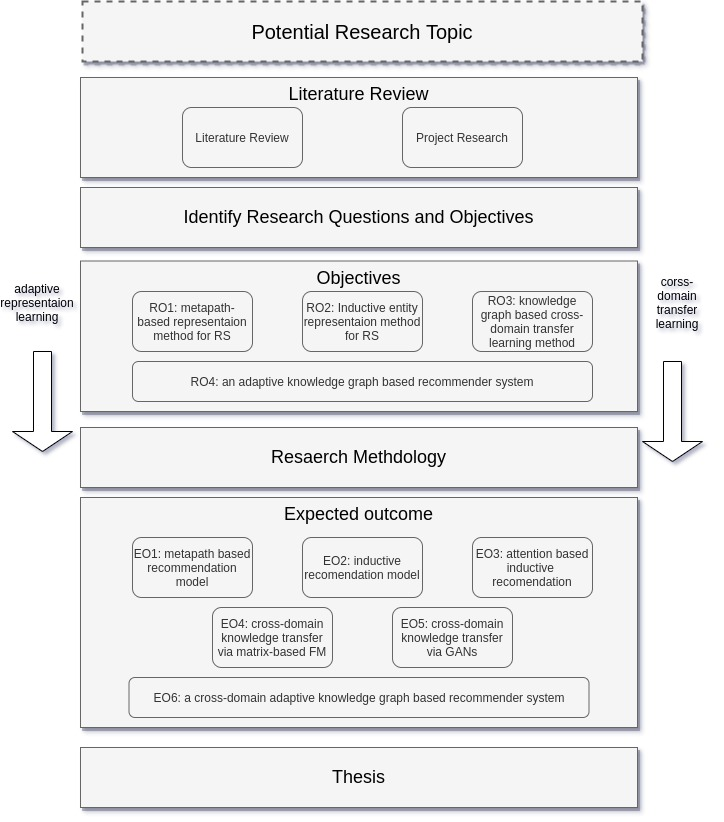
\includegraphics[width=0.99\textwidth]{figs/research_overview.jpg}
    \caption{overview of research perspective}\label{fig:r_overview}
\end{figure*}
